%\documentclass[a4paper,twoside,11pt]{report}
\documentclass[a4paper,singleside,11pt]{report}

\usepackage{ia_urb_thesis}
\usepackage[italian]{babel}
\usepackage[latin1]{inputenc}
\usepackage[T1]{fontenc}
%\usepackage{lmodern}
\usepackage{amsmath,
	    amsfonts,
	    amstext,
	    amssymb,
	    mathrsfs,
	    stmaryrd,
	    latexsym,
	    %enumitem,
	    proof,
	    graphicx,
	    epsfig,
	    color,
	    %hyperref,
	    comment}
%\usepackage{listings}
\begin{document}

\titolo{Creazione di un Gestore di messaggi per la \\[5mm]
        somministrazione di test in Erlang}
\candidato{Paride Dominici}
\relatore{Chiar.mo Prof.~Claudio Antares Mezzina}
%\correlatori{Chiar.mo Prof.~Davide Verdi \\
%             Dott.~Giuseppe Gialli}
\correlatore{Chiar.mo Prof.~Alessandro Aldini} 
\annoaccademico{2024-2025}

\copertinatesi 
\dedica{Alla mia famiglia}
\indice
\indicefigure
\indicetabelle
\iniziatesto

\chapter{Introduzione}

Provo a scrivere nel capitolo



\chapter{Analisi dei requisiti}

\section{Comunicazione}
La prima cosa che dobbiamo analizzare \`e la tipologia di messaggi che possono essere scambiati tra il gestore dei messaggi, i client e il server che gestisce i test.

Per avere un riferimento stiliamo innanzitutto un elenco dei messaggi che potrebbero essere scambiati tra il server e i client in una situazione standard.
\subsection{Esempi di messaggi che possono essere utilizzati}
\begin{itemize}
	\item Registrazione nuova postazione
	\item De-registrazione postazione
	\item Richiesta codice di accesso
	\item Invio codice di accesso
	\item Richiesta invio dati studente
	\item Invio dati studente
	\item Richiesta test da somministrare
	\item Invio contenuto del test da somministrare
	\item Invio risposte test
	\item Termine forzato del test
	\item Mostra messaggio sulla postazione
	\item Richiesta stato postazione
\end{itemize}
\subsection{Requisiti tecnici}
Per poter poter comunicare sia lato client che lato server, visto che le comunicazioni avvengono gi\`a su http o https non useremo erlang direttamente ma ci affideremo al web server Yaws \cite{web:yaws} che \`e stato implentato proprio in Erlang e che permette di inserire all'interno del codice html, in modo simile a PHP, direttamente chiamate a codice Erlang.
Saremo costretti ad adattare il codice del client e del server in modo che comunichino attraverso il nuovo gestore dei messaggi.

\section{Differenze tra le due modalit\`a}
La differenza principale, nella comunicazione tra client e server \`e che nella configurazione originale, senza il gestore dei messaggi, ogni richiesta del client viene gestita direttamente dal server che risponde, nella stessa connessione, con la pagina o il messaggio relativo.

\begin{figure}[!hbtp]
	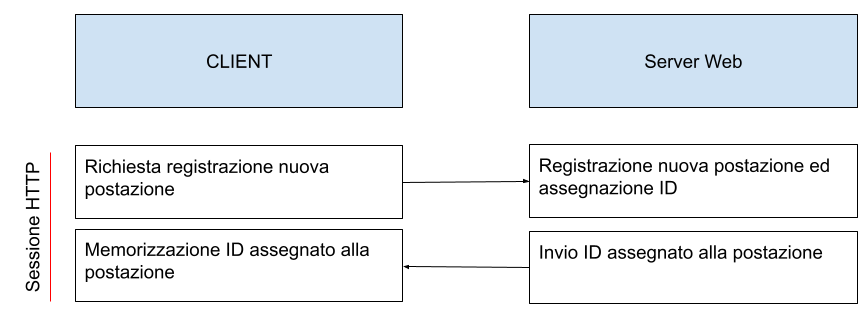
\includegraphics[width=1.0\textwidth]{figure/Disegno 003_ Esempio comunicazione senza gestore messaggi.png}
	\caption{Esempio comunicazione senza gestore messaggi}
	\label{fig:Esempio_comunicazione_senza_gestore_messaggi}
\end{figure}

Nella configurazione con il gestore dei messaggi invece la comunicazione avviene in modo asincrono. Il client fa una richiesta al gestore dei messaggi, questo risponde nella stessa comunicazione con l'ID con il quale la richiesta \`e stata memorizzata nella coda dei messaggi in modo che il client possa sapere quando la richiesta \`e stata processata.

Ad intervalli regolari il client far\`a una richiesta al gestore dei messaggi per conoscere l'esito della sua richiesta.

La comunicazione tra gestore dei messaggi e server PHP avverr\`a in modo simile.
Il gestore dei messaggi prender\`a uno dei messaggi dalla coda e si colleger\`a al server PHP. Per evitare le congestioni implementeremo un sistema che limiti il numero di processi contemporanei attivi. Se tutte le connessioni che abbiamo deciso fossero gi\`a occupate il gestore di messaggi metter\`a il messaggio di nuovo nella coda ed attendender\`a un tempo variabile prima di tentare nuovamente.

Se la connessione va a buon fine il server PHP ci risponder\`a con il risultato della richiesta. Questa verr\`a nuovamente memorizzata nella coda dei messaggi come risposta pronta per essere inviata al client corrispondente all'ID della richiesta originale.

Nel caso della comunicazione con il server avremo una comunicazione sincrona anzich\`e asincrona.

\begin{figure}[!hbtp]
	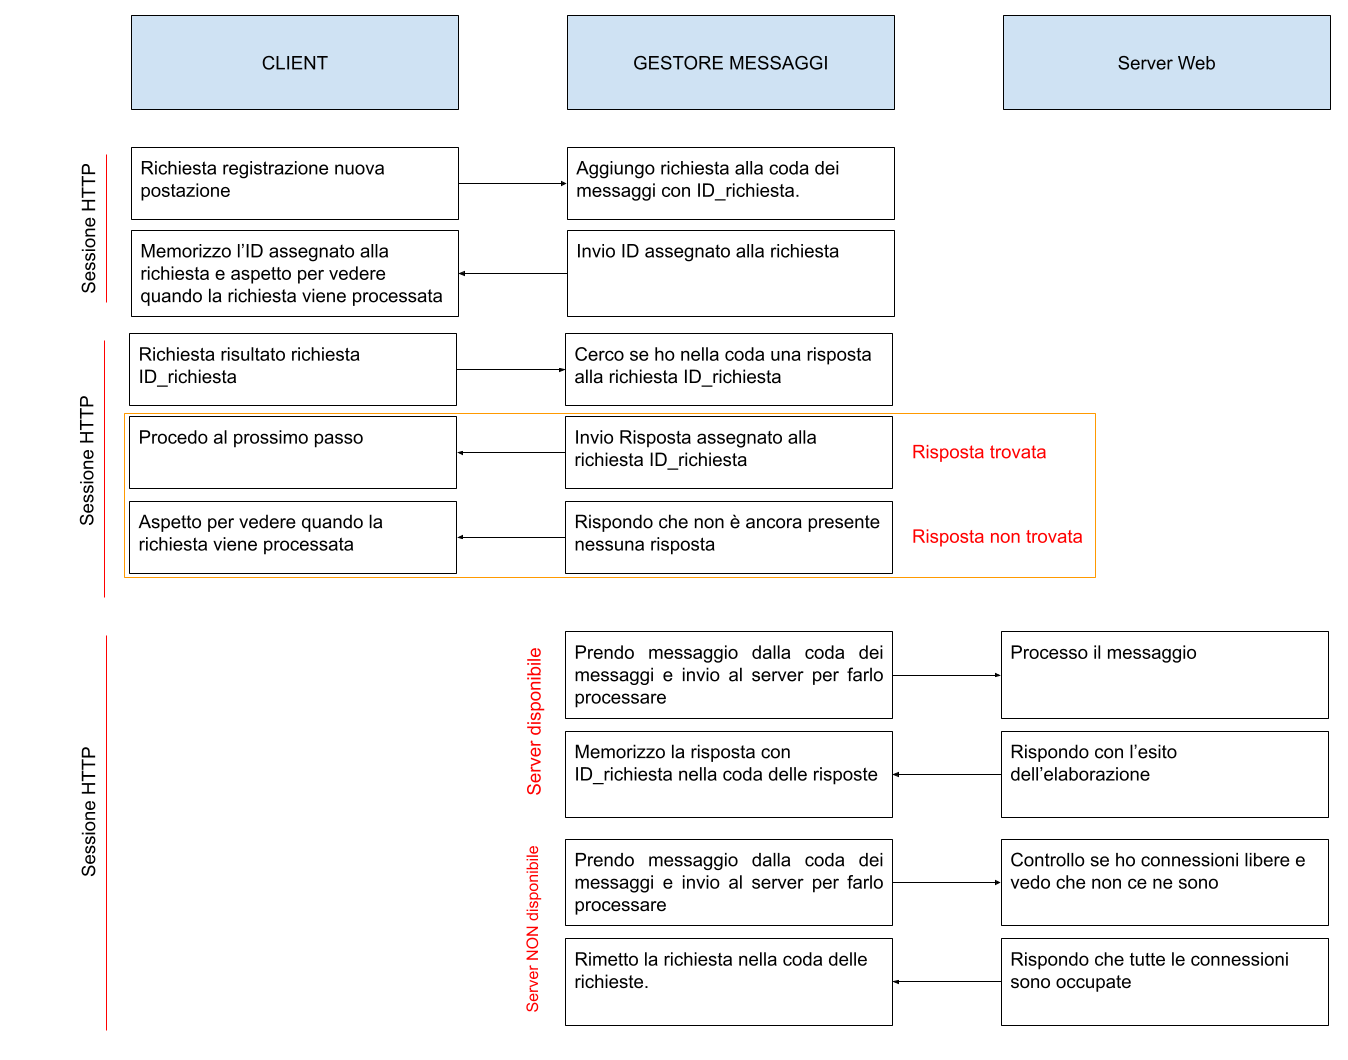
\includegraphics[width=1.0\textwidth]{figure/Disegno 004_ Esempio comunicazione con gestore messaggi}
	\caption{Esempio comunicazione con gestore messaggi}
	\label{fig:Esempio_comunicazione_con_gestore_messaggi}
\end{figure}


\section{Diagrammi degli stati}
Per comprendere meglio quali sono i messaggi che saranno necessari per la comunicazione con il server useremo dei diagrammi degli stati.

\begin{figure}[!hbtp]
	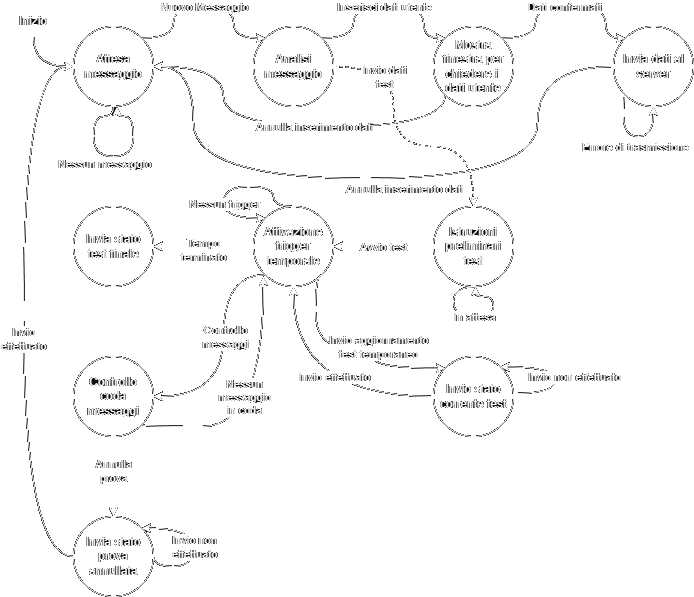
\includegraphics[width=1.0\textwidth]{figure/diagramma_degli_stati_client.png}
	\caption{Diagramma degli stati del Client}
	\label{fig:diagramma_stati_client}
\end{figure}

Sul client, per l'esecuzione di un test la sequenza delle operazioni che questo dovr\`a eseguire \`e la seguente:

\begin{enumerate}
	\item Registrazione postazione sul server PHP*
	\item Inserimento del codice della prova da svolgere nella pagina web da parte dell'utente
	\item Invio richiesta dati del test in base al codice inserito*
	\begin{itemize}
		\item Se il codice non \`e corretto scrivo Codice non corretto e lo faccio inserire di nuovo
		\item Se il codice \`e corretto usa i dati ricevuti dal server per creare dinamicamente la pagina web in base alle caratteristiche del test
	\end{itemize}
	\item Avvio i timer per lo svolgimento del test 
	\begin{itemize}
		\item Invio dello stato temporaneo del test (ogni 30s)*
		\item Controllo se ci sono messaggi o azioni richieste dal server ( interruzione test, messaggio a video, ecc.)*
	\end{itemize}
	\item Consegna test definitivo*
	\begin{itemize}
		\item Consegna manuale prima della scadenza
		\item Consegna per scadenza del tempo
	\end{itemize}
	\item Cancellazione registrazione della postazione*
\end{enumerate}
* vuol dire che c'\`e una richiesta HTTP

\section{Perch\'e scegliere Erlang}
Erlang \`e, come indicato anche nella pagina del progetto \cite{web:erlang}, un linguaggio usato per costruire sistemi soft real-time. massivamente scalabili con requisiti di alta disponibilit\`a. Alcuni dei suoi utilizzi riguardano le telecomunicazioni, il settore bancario, l'e-commerce, la telefonia computerizzata e la messaggistica istantanea. Il sistema di runtime di Erlang dispone di un supporto integrato per la concorrenza, la distribuzione e la tolleranza ai guasti.

Il motivo principale per cui l'ho scelto \`e la sua capacit\`a di scalare usando una quantit\`a minima di risorse. Inoltre pu\`o lavorare in modo distribuito su pi\`u macchine e pu\`o, in caso di errori nell'esecuzione del programma, ripristinare l'esecuzione in modo automatico.

\subsection{Erlang/OTP}
OTP che sta per Open Telecom Platform \`e un framework di sviluppo e una collezione di librerie, componenti di design e middleware che permettono di strutturare applicazioni Erlang in modo robusto e standardizzato.

OTP fornisce dei modelli pronti all'uso per gestire i compiti pi\`u comuni come ad esempio:
\begin{itemize}
	\item \textbf{gen\_server} - Per implementare la logica client-server
	\item \textbf{gen\_statem} - Per gestire macchine a stati finiti
	\item \textbf{supervisor} - Fondamentale per la tolleranza ai guasti (monitora altri processi e li riavvia se falliscono
\end{itemize}

Un concetto fondamentale di Erlang/OTP \`e l'albero di supervisione (\textit{supervision tree}). Questo \`e una modalit\`a di strutturazione del modello basato sull'uso di \textit{workers} e \textit{supervisors}.

\begin{itemize}
	\item I \textit{worker} sono i processi che svolgono effettivamente il lavoro.
	\item I Supervisori (\textit{supervisors}) sono processi che monitorano i \textit{worker} e fanno li fanno ripartire se ci sono problemi. 
\end{itemize}

L'albero di supervisione (\textit{supervision tree}) \`e una organizzazione gerarchica del codice in supervisori e worker che ci permette di progettare sistemi che sono resistenti ai guasti (\textit{fault-tolerant}).

\begin{figure}[!hbtp]
	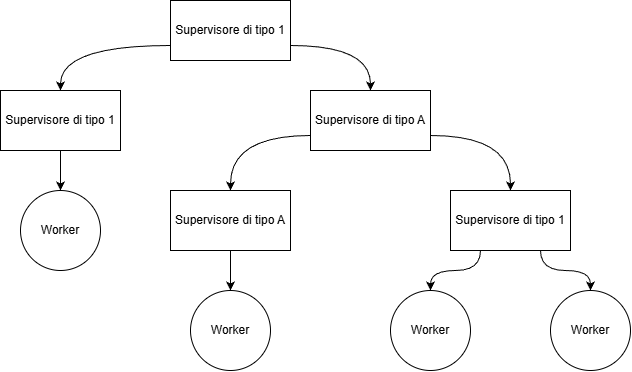
\includegraphics[width=1.0\textwidth]{figure/Erlang-OTP Supervision Tree.png}
	\caption{Supervision Tree}
	\label{fig:erlang-otp-supervision-tree}
\end{figure}

Una cosa molto interessante \`e che i supervisori e i worker possono essere sulla stessa macchina ma possono anche essere messi su macchine diverse. Questo ci permette di garantire che, anche se il problema riguarda fisicamente una macchina, il sistema pu\`o continuare a funzionare, creando nuovi nodi che svolgano i compiti che venivano svolti sulla macchina non pi\`u funzionante.

\subsection{Invio e ricezione di messaggi}
Altra caratteristica estremamente interessante di Erlang \`e la gestione nativa dei messaggi.

I vari processi (attori), infatti, possono comunicare tra di loro con un sistema di messaggistica nativo del linguaggio. Ad esempio per inviare un messaggio ad un altro processo \`e sufficiente il comando:

\begin{verbatim}
Pid ! Messaggio
\end{verbatim} 

Dove \textit{Pid} \`e l'id del processo a cui inviare il messaggio.

Per ricevere messaggi, un processo utilizza il blocco receive, che analizza la "cassetta postale" (mailbox) del processo stesso.

\begin{verbatim}
receive
    Pattern1 -> Azioni1;
    Pattern2 -> Azioni2
end
\end{verbatim} 

a seconda del \textit{pattern} ricevuto verr\`a eseguita l'azione corrispondente. 

\subsection{Hot Code Swapping}
Un'altra caratteristica interessante di erlang rispetto ad altri linguaggi \`e la sua capacit\`a di aggiornare il codice di una applicazione mentre questa \`e in esecuzione (\textit{Hot Code Swapping}), senza interrompere il servizio. I nuovi processi utilizzeranno il nuovo codice, mentre quelli vecchi continueranno con la versione precedente finch\`e non terminano o vengono aggiornati.


\subsection{Casi d'uso - Whatsapp}
Erlang \`e estremamente efficente e ne abbiamo prova, ad esempio, dal fatto che la gestione di messaggi dell'applicazione di messaggistica \textit{Whatsapp} viene fatta utilizzando le macchine virtuali BEAM di Erlang.

La capacit\`a di gestire una elevata concorrenza permette ad ogni server di gestire fino a 2 milioni di connessioni contemporanee. Questo gli permette, con un team estremamente ridotto, di gestire tranquillamente oltre 100 miliardi di messaggi al giorno mantenendo, grazie alla struttura \textit{fault-tolerant}, una enorme affidabilit\`a e tolleranza ai guasti.





\chapter{Strutture di comunicazione}
La comunicazione tra il client, il gestore dei messaggi e il server avvengono attraverso strutture json.
\section{Struttura JSON}
La struttura JSON che viene inviata per la comunicazione tra i vari elementi dovr\'a avere uno schema del tipo:
\begin{verbatim}
{
  msg_type: tipo_messaggio,
  msg_content: contenuto_del_messaggio
}
\end{verbatim}

I messaggi di ritorno avranno una struttura del tipo:

\begin{verbatim}
{
  result_type: tipo_messaggio_di_ritorno,
  result_content: contenuto_del_messaggio
}
\end{verbatim}

Codifichiamo quindi i messaggi per il gestore dei messaggi:

\begin{tabular}{|c|l|}
	\hline
	test\_messaggio & Serve per fare un semplice test di comunicazione\\
	\hline
	register\_station & Indica al sistema che la postazione vuole essere registrata sul sistema \\
	\hline
	unregister\_station & Indica al sistema che la postazione vuole essere tolta dal sistema \\
    \hline
	request\_code & Indica al sistema che la postazione vuole essere registrata sul sistema \\
    \hline
	register\_station & Indica al sistema che la postazione vuole essere registrata sul sistema \\
    \hline
\end{tabular}


\chapter{Implementazione in Erlang}
Per l'implementazione ci affideremo al web server implementato in Erlang\cite{web:erlang},  Yaws\cite{web:yaws}. 

Yaws usa un sistema simile a quello di PHP.
Permette infatti di includere codice erlang direttamente all'interno della pagina WEB inserendolo all'interno delle coppia di tag <erl> e </erl>.

\chapter{Verifica della funzionalit\'a}
\chapter{Conclusioni}

Dopo aver effettuato le prove possiamo concludere che l'idea dell'utilizzo di un gestore di messaggi per rendere pi\`u efficente e robusto il server PHP \`e realizzabile.

Durante la creazione del progetto sono emerse alcune criticit\`a e soluzioni alternative che potrebbero essere implementate sfuttando una buona parte del codice gi\`a scritto.

Una grossa criticit\`a di Yaws \`e che il codice erlang deve essere all'interno della stessa pagina ed \`e difficile, se non facendo operazioni particolari, usare dei moduli esterni personalizzati. Questo risulta in un codice molto lungo e poco leggibile e rende anche la manutenzione stessa dei moduli pi\`u difficoltosa.

Per quanto riguarda i miglioramenti, si potrebbe ad esempio, come citato nel capitolo 4.3.2, creare un collegamento tra la VM erlang di Yaws e altre esterne ad esso e, condividendo il database con macchine diverse da quella su cui gira il Web server Yaws, aumentarne la resilienza ed affidabilit\`a.

Un passo in avanti, utilizzando sempre il server Yaws, potrebbe essere quella di spostare tutta la parte di elaborazione dati e scrittura e lettura dei dati nella tabella mnesia, sul codice Erlang nativo e di usare il web server solo per l'accesso da parte dei client. Potremmo in questo caso sfruttare la messaggistica interna di Erlang per inviare le richieste ricevute dai client ai vari attori (worker). In questo modo riusciamo ad alleggerire il carico sul Single Point Of Failure che nel nostro caso \`e il Web Server Yaws.

Un ultimo miglioramento che si potrebbe fare \`e di riscrivere completamente la parte di gestione delle chiamate web direttamente nel nostro codice senza utilizzare il server Yaws. In questo caso il vantaggio sarebbe che non \`e necessario modificare la configurazione del web server per renderlo parte della rete Erlang. Anche in questo caso, buona parte del codice che abbiamo gi\`a scritto potrebbe essere riutilizzato.

Il fatto di avere tutto in Erlang nativo ci permette anche di superare la limitazione dettata da Yaws e dividere il nostro codice in diversi moduli rendendolo pi\`u leggibile e manutenibile.

In conclusione, nonstante Erlang sia un linguaggio un po' ostico a causa della sua sintassi e del modo in cui alcune strutture della programmazione devono essere ripensate per poter essere implementate, la sua efficienza lo rende il linguaggio pi\`u adatto per progetti di questo tipo.


	
%\include{sorgenti/cap_7}
%\include{sorgenti/cap_8}

\appendix
\chapter{Appendice A}


\section{Client javascript per Verifica connessione di base}
\label{javascript_verifica_base_src}
\begin{verbatim}
<html>
<head>
<title>Client</title>
<link rel="icon" type="image/png" href="/favicon.png"> 
<link rel="shortcut icon" href="/favicon.ico">
</head>
<body>
<h1>Client di prova per verificare la comunicazione automatica con il 
gestore di messaggi</h1>

<p><a href="javascript:StartInvioMessaggi()">Inizia invio dei messaggi 
al gestore messaggi.</a></p>
<p>Test get Yaws: <span id="get"></span></p>
<p>Test get PHP: <span id="get_php"></span></p>

<div>Test POST con parametri Yaws: <span id="post_parametri"></span></div>
<div style="border: 1px solid black;" id="return_message"></div>
<div>Test POST con parametri PHP: <span id="post_parametri_php"></span></div>
<div style="border: 1px solid black;" id="return_message_php"></div>

<script src="utils.js">	</script>
<script>		
var server = "http://localhost:8080/server.yaws";
var server_php = "http://localhost/server.php";

var t_invio_messaggi;
var invio_messaggi_refresh_time_first_time = 1 * 1000; /* x secondi */
var invio_messaggi_refresh_time = 10 * 1000; /* x secondi */
var numero_iterazioni = 0;

	/* Inizializza la procedura per inviare i messaggi ai server */
	function StartInvioMessaggi() {
		clearTimeout(t_invio_messaggi);
		t_invio_messaggi = setTimeout('InvioMessaggi()',
		           invio_messaggi_refresh_time_first_time); 
	}

	/* Funzione che invia un messaggio ai server */
	function InvioMessaggi()
	{
		const dati = 
		{ 
			"msg_type": "test_message", 
			"msg_content": {
				"numero_iterazioni": numero_iterazioni, 
				"test": "Sara" 
			}
		};
		numero_iterazioni = numero_iterazioni + 1;
		
		/* invio un messaggio di tipo POST al server Yaws */	
		post(server, dati).then((post_res) => {
			document.getElementById("post_parametri").innerHTML =
							post_res.risposta.result_type;
			document.getElementById("return_message").innerHTML = 
							post_res.risposta.result_content;
			console.log("msg-arrived:" + post_res.risposta.result_type);
			console.log("post_res :" + post_res.risposta.result_content);
		});
		
		post(server_php, dati).then((post_res) => {
			document.getElementById("post_parametri_php").innerHTML = 
							post_res.risposta.result_type;
			document.getElementById("return_message_php").innerHTML = 
							post_res.risposta.result_content;
			console.log("msg-arrived_php:" + post_res.risposta.result_type);
			console.log("post_res_php:" + post_res.risposta.result_content);
		});
		
		/* faccio ripartire il timer per la prossima iterazione */
		t_invio_messaggi = setTimeout('InvioMessaggi()', invio_messaggi_refresh_time); 
	}

	/* invio un messaggio di tipo GET al server Yaws */	
	get(server).then((post) => {
		document.getElementById("get").innerHTML = post.result;
	});
	
	/* invio un messaggio di tipo GET al server php */	
	get(server_php).then((post) => {
		document.getElementById("get_php").innerHTML = post.result;
	});

	</script>
	</body>
	</html>

\end{verbatim}

\begin{thebibliography}{widestlabel}
 	\bibitem{art:erlang}Francesco Cesarini e Simon Thompson,
	\emph{Erlang Programming}, 
	United States of America: O'Reilly, 
	2009	
	
	\bibitem{art:building_web_erlang}Zachary Kessin,
	\emph{Programming Web Services with Erlang: Working with Yaws}, 
	Great Britain: O'Reilly, 
	2012	
	
	

	\bibitem{web:erlang}
	\emph{Index - Erlang/OTP} [Online] (26/11/2025). [Ultimo Accesso: 26/11/2025]. 
	Disponibile: https://www.erlang.org/
	
	\bibitem{web:elixir}
	\emph{The Elixir programming language} [Online] (28/12/2025). [Ultimo Accesso: 28/12/2025]. 
	Disponibile: https://elixir-lang.org/

	
	
	\bibitem{web:yaws}
	\emph{Yaws (web server) - Wikipedia} [Online] (28/12/2025). [Ultimo Accesso: 28/12/2025]. 
	Disponibile: https://en.wikipedia.org/wiki/Yaws\_(web\_server)
	
	
\end{thebibliography}

\ringraziamenti
Desidero ringraziare il mio relatore, il Prof. Claudio Antares Mezzina, per la guida e la costante disponibilit� durante lo sviluppo di questo lavoro.

Un sentito ringraziamento va al correlatore, il Prof. Alessandro Aldini, per il prezioso supporto e le osservazioni fornite.

Estendo la mia gratitudine a tutti i docenti del corso di laurea per gli insegnamenti ricevuti e per aver contribuito alla mia formazione accademica in questi anni.

Ringrazio i miei amici e colleghi per il sostegno e la condivisione di questo percorso.

Infine, un ringraziamento speciale alla mia famiglia per il supporto incondizionato che ha reso possibile questo traguardo.

\end{document}
